\documentclass{jsarticle}
\usepackage[dvipdfmx]{graphicx}
\usepackage{listings,jlisting}
\lstset{%
  language={C},
  basicstyle={\small\ttfamily},%
  identifierstyle={\small},%
  commentstyle={\small\itshape},%
  keywordstyle={\small\bfseries},%
  ndkeywordstyle={\small},%
  stringstyle={\small\ttfamily},
  frame={tb},
  breaklines=false,
  columns=[l]{fullflexible},%
  numbers=left,%
  xrightmargin=0zw,%
  xleftmargin=3zw,%
  numberstyle={\scriptsize},%
  stepnumber=1,
  numbersep=1zw,%
  lineskip=-0.5ex%
}

\begin{document}

\title{画像工学 レポート\\ \vspace{1cm}― pgmファイルの解析とヒストグラム生成 ―\vspace{2cm}}
\author{IE5 (9) 片岡 駿之介 \vspace{1cm}}
\maketitle

\newpage

\section{課題}

PGMは画像フォーマットPNM\cite{ref1}の一種で,グレースケールを表現できる形式となっている.PGMは「portable graymap format」と呼ばれている.PNMには他にも2値画像,RGB画像に対応したものも存在し,それぞれPBM,PPMと呼ばれている.\\
本レポートでは,PGM画像のヘッダから画像のメタデータを取得した後に画像データ部を解析し,それによってヒストグラムを生成する.

\section{解析}

今回の演習では,PGMファイルを以下の手順で解析していくこととした.
\begin{enumerate}
  \item 入力されたコマンドが正しいかチェック(正しくない場合はUsageを表示して終了)
  \item コマンドで指定されたPGMファイルを読み込む
  \item 読み込んだPGMファイルのヘッダ解析のスタート
  \item マジックナンバーをチェック(マジックナンバーが異なる場合はその旨を表示して終了)
  \item 画像の横のサイズを取得
  \item 画像の縦のサイズを取得
  \item 画像の最大輝度値設定を取得
  \item 以降,画像データの読み込みをスタートし,ヒストグラムを生成
\end{enumerate}

この解析によって得られたヒストグラムのデータをtxtファイルに保存し,gnuplotでプロットを行うことにより,ヒストグラムのグラフを出力する.
\newpage

\section{ソースリスト}

\begin{lstlisting}[caption=histogram.c,label=ほげ]
  #include <stdio.h>
  #include <stdlib.h>
  #include <ctype.h>

  FILE *fp;

  int width;
  int height;
  int max_value;

  int status;
  char buffer[128];

  void image_open(char *file_name) {
    if ((fp = fopen(file_name, "r")) == NULL) {
     printf("file open error!!\n");
     exit(-1);	/* (3)エラーの場合は通常、異常終了する */
   }
    // printf("%s\n", file_name);
  }

  int main(int argc,char *argv[]) {

    /* 入力コマンドのチェック */
    if(argc == 1) {
      printf("Usage : ./histogram <pgm file name>\n");
      exit(0);
    } else if (argc == 2) {
      image_open(argv[1]);
    }

    /* ヘッダ取得部 */
    int ch;

    while (status < 3) {
      ch = getc(fp);

      if(ch == '#') { // コメントのスキップ
        while (( ch = getc(fp)) != '\n')
          break;
      }

      if(ch == 'P') { // マジックナンバーのチェック
        if(getc(fp) != '5') {
          printf("Magic Number is wrong.\n");
          break;
        } else {
          // printf("Magic Number is P5\n");
        }
      }

      if(isdigit((unsigned char)ch)) { // 数値取得部
        buffer[0] = ch;
        int i=1;
        while(1) {
            char c = getc(fp);
            if(isdigit((unsigned char)c)) {
              buffer[i]=c;
              i++;
            } else
              break;
        }
        buffer[i] = '\0';

        switch (status) {
          case 0: // width取得部
            width = atoi(buffer);
            // printf("width=%d\n", width);
            break;
          case 1: // height取得部
            height = atoi(buffer);
            // printf("height=%d\n", height);
            break;
          case 2: // max_value取得部
            max_value = atoi(buffer);
            // printf("max_value=%d\n", max_value);
            break;
        }
        status++; // 次のステータスへ
      }
    }

    /* ヒストグラム生成部 */
    int histogram[1024] = {};

    while ((ch=getc(fp)) != -1) {
      histogram[(int)ch]++;
    }

    for(int k=0; k <= max_value; k++) {
      printf("%4d %5d\n", k, histogram[k]);
    }
  }

\end{lstlisting}

\newpage

\section{結果}
本演習で与えられた2枚のPGMファイル「cup.pgm」と「source.pgm」を図1,図2に示す.
\begin{figure}[htbp]
 \begin{minipage}{0.5\hsize}
  \begin{center}
   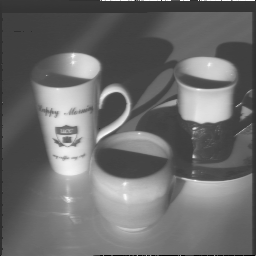
\includegraphics[width=70mm]{cup.png}
  \end{center}
  \caption{cup.pgm}
  \label{fig:one}
 \end{minipage}
 \begin{minipage}{0.5\hsize}
  \begin{center}
   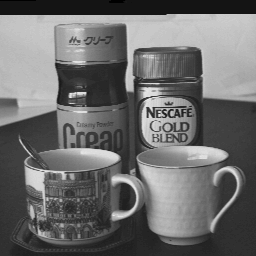
\includegraphics[width=70mm]{source.png}
  \end{center}
  \caption{source.pgm}
  \label{fig:two}
 \end{minipage}
\end{figure}

「2.解析」で示した手順で「cup.pgm」「source.pgm」を解析し,グラフにプロットしたものを図3,図4に示す.\\

\begin{figure}[htbp]
 \begin{minipage}{0.5\hsize}
  \begin{center}
   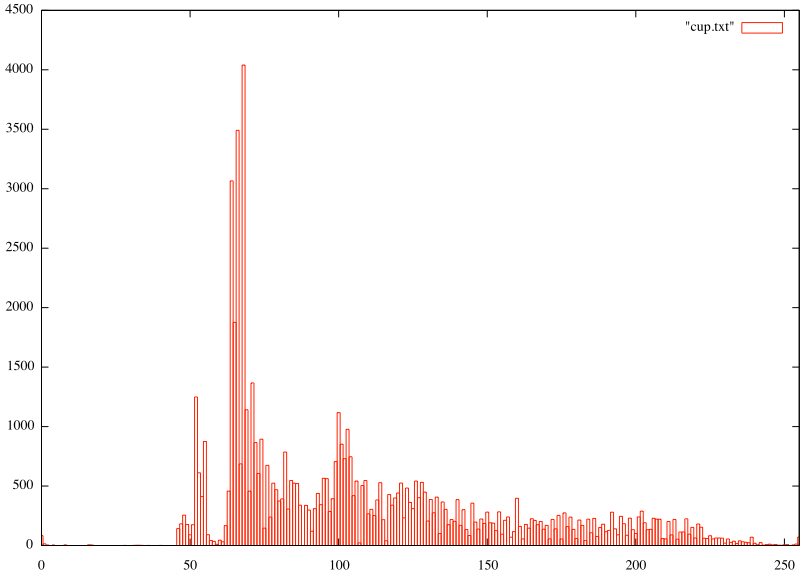
\includegraphics[width=70mm]{cup_histogram.png}
  \end{center}
  \caption{cup.epsのヒストグラム}
  \label{fig:three}
 \end{minipage}
 \begin{minipage}{0.5\hsize}
  \begin{center}
   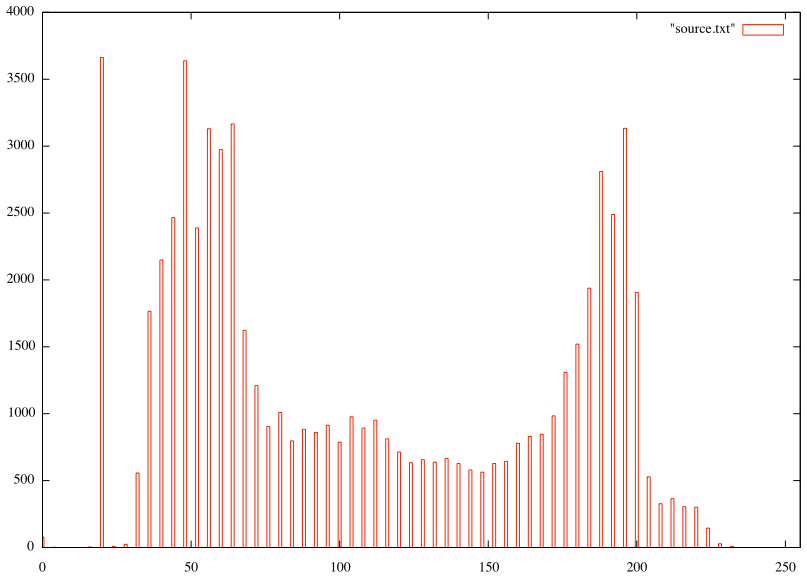
\includegraphics[width=70mm]{source_histogram.png}
  \end{center}
  \caption{source.epsのヒストグラム}
  \label{fig:four}
 \end{minipage}
\end{figure}

\newpage

以下に,画像編集ソフト「GIMP」で2つのPGMファイルを開き,ヒストグラムを観察したものを示す.

\begin{figure}[htbp]
 \begin{minipage}{0.5\hsize}
  \begin{center}
   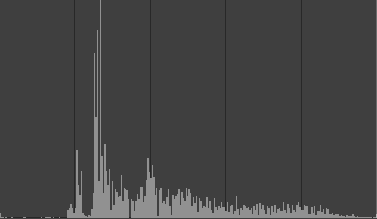
\includegraphics[width=70mm]{cup_gimp_histogram}
  \end{center}
  \caption{cup.epsのヒストグラム(GIMP)}
  \label{fig:five}
 \end{minipage}
 \begin{minipage}{0.5\hsize}
  \begin{center}
   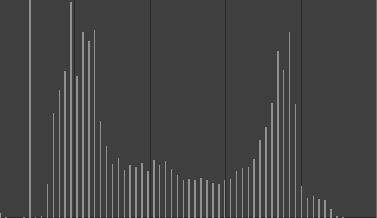
\includegraphics[width=70mm]{source_gimp_histogram.png}
  \end{center}
  \caption{source.epsのヒストグラム(GIMP)}
  \label{fig:six}
 \end{minipage}
\end{figure}

それぞれを見比べると,同一形状のヒストグラムが生成されていることがわかる.

\section{考察}

演習で与えられたPGMファイルは,2つともヘッダの記述フォーマットが少し異なっており,そこを如何に解決するかが本演習の肝だった.\\
PNMフォーマットのヘッダは一番はじめにマジックナンバーが来るという性質を利用してマジックナンバーを確定し,その後は順番に横幅,縦幅,最大輝度値という順番でヘッダを解析するという方針でプログラムを実装した.また,ヘッダに記載されている情報は改行・空白で区切られているため,コメント・改行・空白以外の部分で情報を一度文1字列として取得し,数値に変換するという手法を取った.\\
実際にプログラムを動かしてみると,正しく情報を更に取得できていることが確認できたため,正しく実装できたと考えている.

\section{感想}
最近はRubyやPythonといったスクリプト言語しか書いていなかったので,やはりC言語での文字列操作はつらいという印象を受けた.\\

\begin{thebibliography}{99}
\bibitem{ref1}
	PNM (画像フォーマット) ―  https://ja.wikipedia.org/wiki/PNM\_(画像フォーマット)
\end{thebibliography}

\end{document}
